\subsection{Backend Package Diagram}
The backend code structure is organized into modular packages to isolate concerns and enforce clear boundaries between different components of the FastAPI application. Figure \ref{fig:backend_package} displays the layout of the backend directory:

\begin{figure}[H]
    \centering
    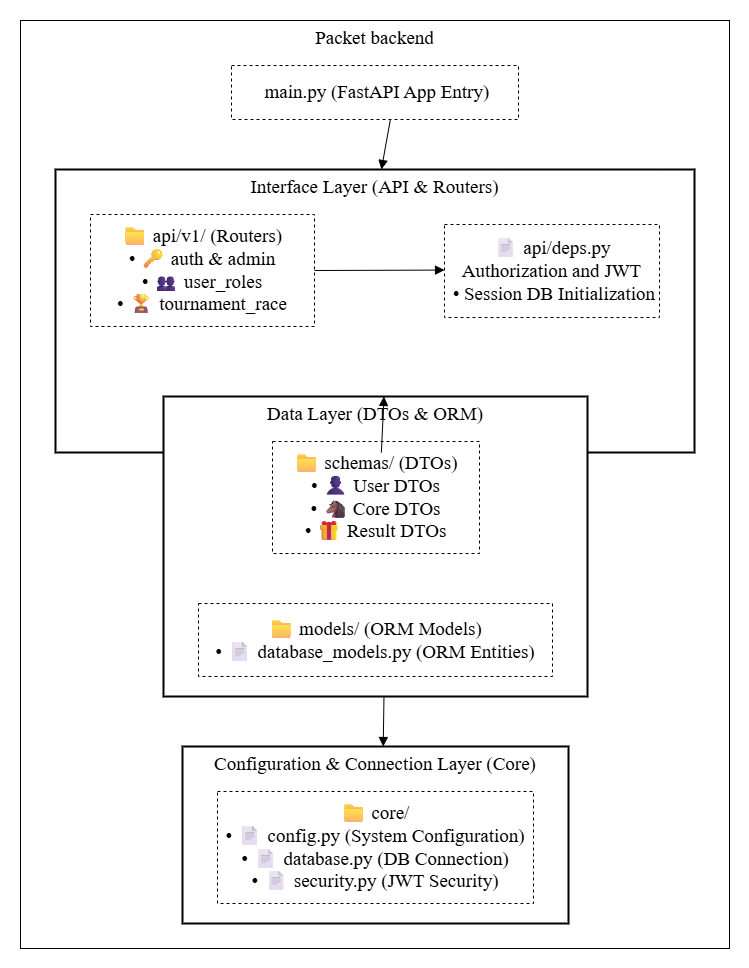
\includegraphics[width=0.9\textwidth]{figures/chuong4_diagram_chung/backend_package.png}
    \caption{Backend Package Structure}
    \label{fig:backend_package}
\end{figure}

The packages and modules are structured as follows:
\begin{itemize}
    \item \textbf{\texttt{api/}:} Houses the API routers. The subpackage \texttt{v1/} contains separate router modules for each logical subdomain (such as authentication, user roles, and tournament/race management). The file \texttt{deps.py} implements dependency injection providers.
    \item \textbf{\texttt{schemas/}:} Defines Pydantic data serialization models (DTOs) representing the structured format of requests and responses for all major subdomains (user, horse, race, prize, result, tournament).
    \item \textbf{\texttt{models/}:} Contains SQLAlchemy declarative models (\texttt{database\_models.py}) mapped to the physical database tables.
    \item \textbf{\texttt{core/}:} Holds core system modules, including system configurations (\texttt{config.py}), JWT security utilities (\texttt{security.py}), and database connection managers (\texttt{database.py}).
\end{itemize}

\subsection{Web Application Package Diagram}
The frontend codebase is organized using the Next.js App Router structure. Figure \ref{fig:web_package} displays the frontend package structure:

\begin{figure}[H]
    \centering
    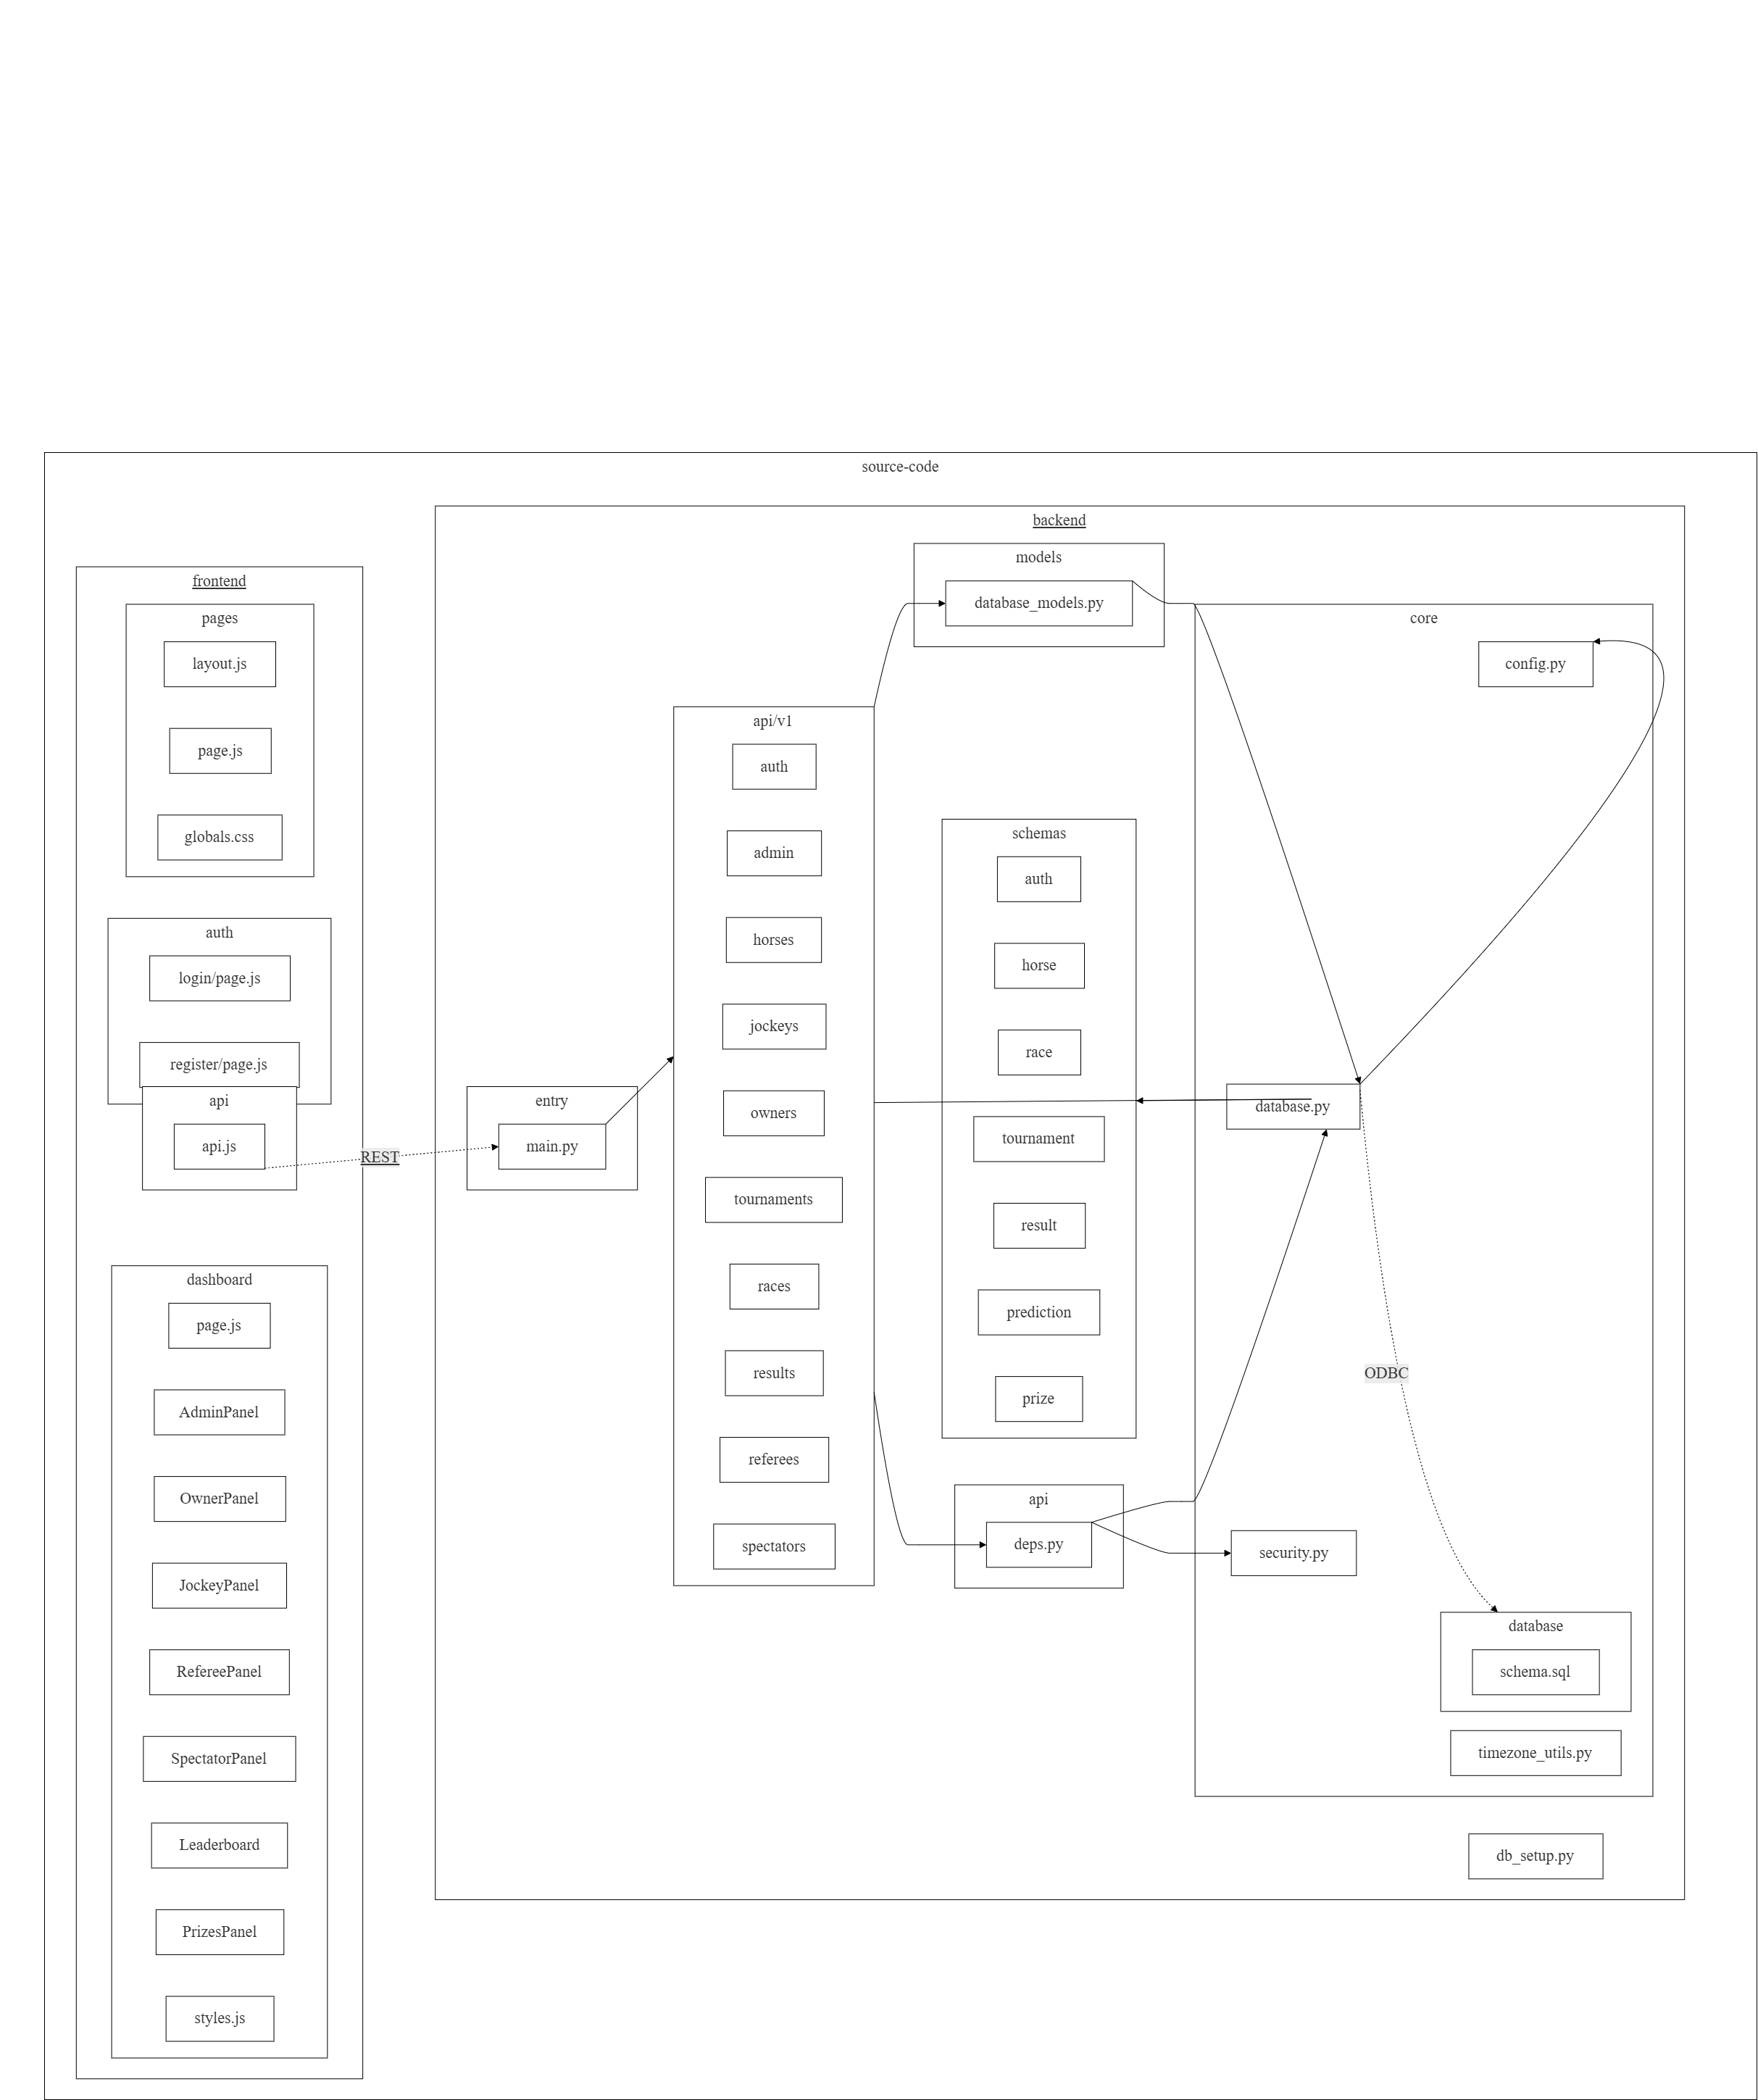
\includegraphics[width=0.9\textwidth]{figures/chuong4_diagram_chung/web_package.png}
    \caption{Web Application Package Structure}
    \label{fig:web_package}
\end{figure}

The major frontend modules are organized inside the following directories:
\begin{itemize}
    \item \textbf{\texttt{app/}:} Root of the application router. The files \texttt{layout.js} and \texttt{page.js} render the root layout and landing page. The file \texttt{api.js} contains utility methods for interacting with the backend API.
    \item \textbf{\texttt{login/} and \texttt{register/}:} Route directories managing authentication pages.
    \item \textbf{\texttt{dashboard/}:} Route directory for the dashboard. It contains the controller \texttt{page.js} and a subfolder \texttt{components/} that groups the role-specific interface panels (Admin, Referee, Jockey, Owner, Spectator).
\end{itemize}
